This section addresses the research question: \textit{Which seasonal windows and locations optimize safety—combining sunshine hours, wind-gust flags, and frost/heat indicators?}

\subsubsection{Calculation Method}

The safety score is a composite metric designed to evaluate environmental
safety conditions for each weather station across Austria, using data from the
last five years only. It combines the following variables:

\begin{itemize}
    \item \textbf{Average Sunshine Hours}: Higher values are considered favorable.
    \item \textbf{Frequency of Wind Gusts}: Higher values are penalized due to increased hazard potential.
    \item \textbf{Frequency of Frost Days}: Higher values indicate harsher conditions and are penalized.
    \item \textbf{Frequency of Heat Days}: Moderately penalized to reflect discomfort and potential risk.
\end{itemize}

The score is calculated as a weighted sum:

\begin{equation}
    \text{Score} = \text{Sunshine} - \text{Wind Gust Freq} - \text{Frost Freq} - \text{Heat Freq}
\end{equation}

A higher safety score indicates more favorable and stable environmental
conditions. The score is then robustly normalized, clipped to a range, and
scaled to 0–100 for comparability.

\subsubsection{Top Station Scores}

Number of stations used: 1134.

Table~\ref{tab:top_scores} lists the top 10 station-season combinations ranked
by safety score within the last five years. These stations span multiple
Bundesländer and elevation zones, demonstrating consistently high safety
scores.

\begin{table}[H]
    \centering
    \begin{tabular}{|c|c|c|c|c|c|c|c|}
        \hline
        \textbf{ID} & \textbf{Season} & \textbf{Region} & \textbf{Elevation} & \textbf{Avg Sun} & \textbf{Safety Score}         \\
        \hline
        25          & Winter          & Stmk            & 1000–1499 m        & 38.0 h                                             & 100.0 \\
        205         & Spring          & OÖ              & 1500–1999 m        & 85.94 h                                            & 100.0 \\
        82          & Winter          & Sbg             & 2000+ m            & 177.59 h                                           & 100.0 \\
        66          & Spring          & T               & 1500–1999 m        & 75.13 h                                            & 100.0 \\
        173         & Winter          & Vlg             & 1000–1499 m        & 38.0 h                                             & 100.0 \\
        82          & Spring          & Sbg             & 2000+ m            & 228.75 h                                           & 100.0 \\
        88          & Winter          & NÖ              & 500–999 m          & 41.81 h                                            & 100.0 \\
        68          & Winter          & Sbg             & 1500–1999 m        & 141.25 h                                           & 100.0 \\
        213         & Winter          & Sbg             & 2000+ m            & 221.76 h                                           & 100.0 \\
        82          & Summer          & Sbg             & 2000+ m            & 43.20 h                                            & 100.0 \\
        \hline
    \end{tabular}
    \caption{Top 10 Safety Scores by Station and Season (Last 5 Years)}
    \label{tab:top_scores}
\end{table}

\subsubsection{Visual Interpretation}

\begin{figure}[H]
    \centering
    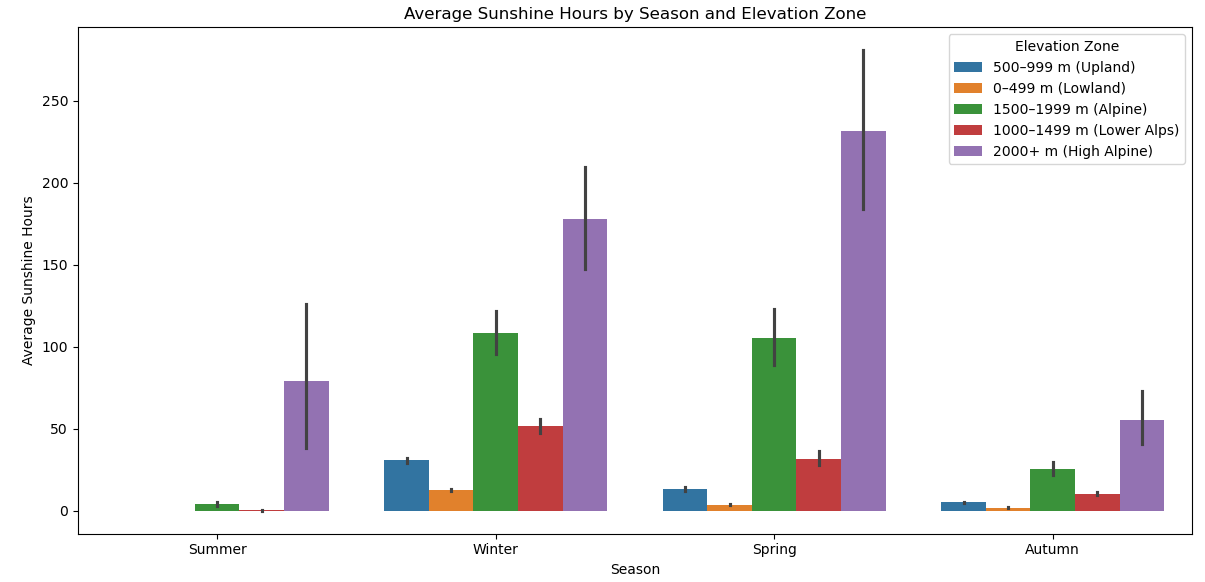
\includegraphics[width=0.45\textwidth]{img/sunshine_by_season_zone.png}
    \caption{Average Sunshine Hours by Season and Elevation Zone (Last 5 Years)}
    \label{fig:sunshine}
\end{figure}

Figure~\ref{fig:sunshine} shows the high alpine zone consistently records
higher average sunshine hours across all seasons, especially in spring,
contributing positively to their safety scores.

\begin{figure}[H]
    \centering
    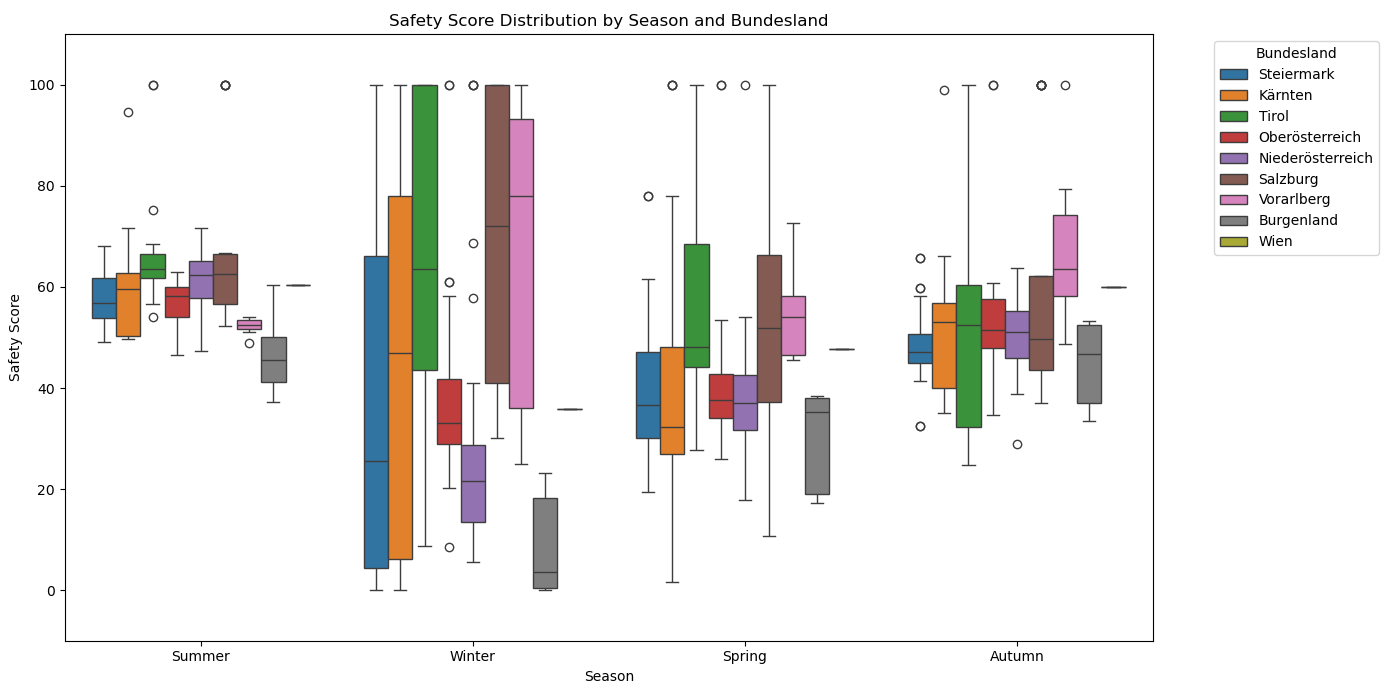
\includegraphics[width=0.45\textwidth]{img/safety_score_boxplot.png}
    \caption{Safety Score Distribution by Season and Bundesland (Last 5 Years)}
    \label{fig:safety_boxplot}
\end{figure}

Figure~\ref{fig:safety_boxplot} presents the distribution of safety scores
filtered to recent years. Salzburg, Tirol, and Vorarlberg show the highest
spread and highest values in winter and spring, corresponding to high-elevation
stations.

\begin{figure}[H]
    \centering
    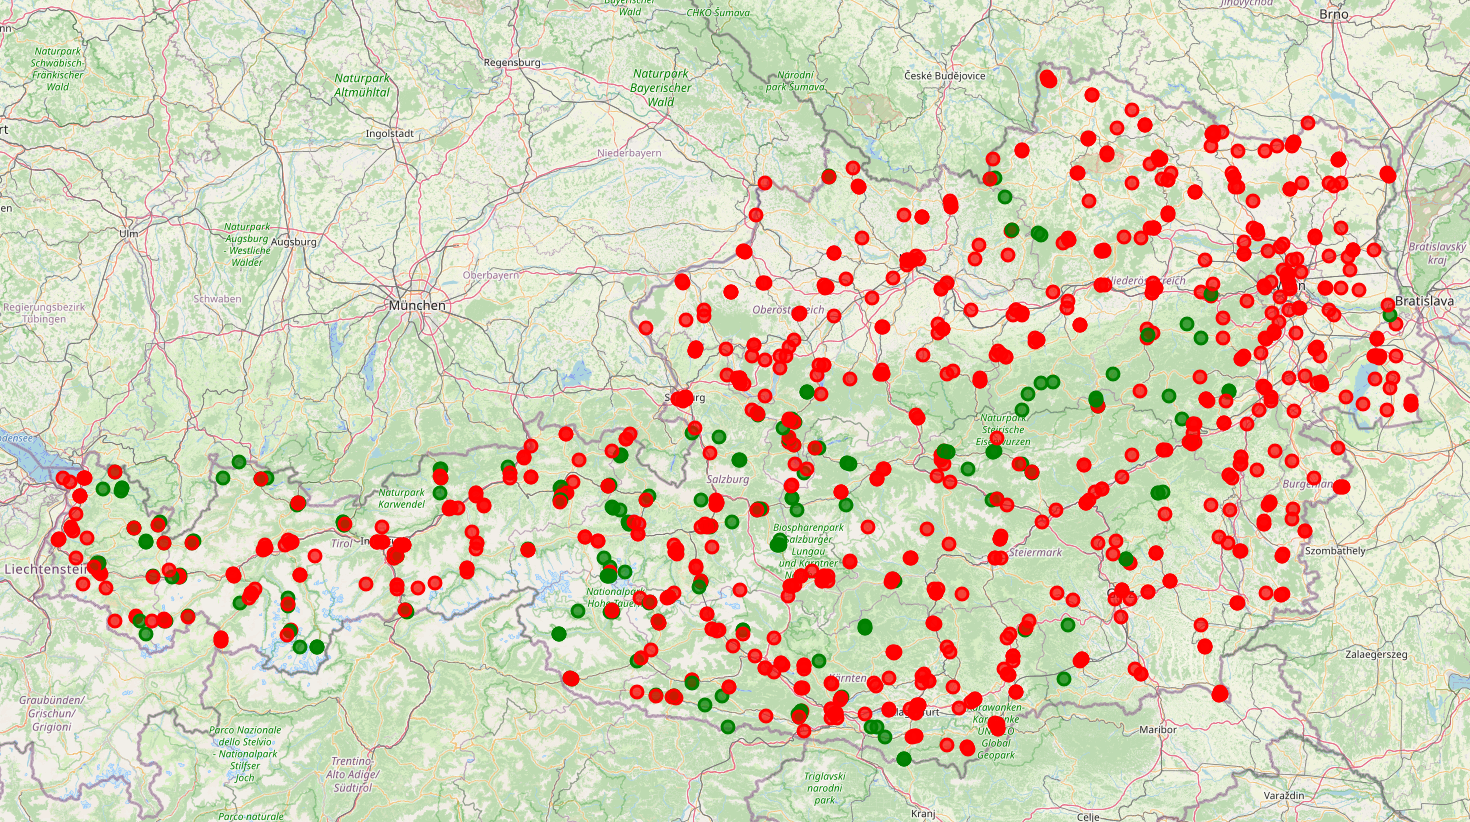
\includegraphics[width=0.45\textwidth]{img/station_map.png}
    \caption{Map of Stations by Safety Score (Green: High, Red: Low, Last 5 Years)}
    \label{fig:station_map}
\end{figure}

Figure~\ref{fig:station_map} visualizes the spatial distribution of safety
scores over the last five years. Green points indicate stations with relatively
high safety scores, predominantly in Alpine regions. Red points represent
stations with lower scores, more frequent in lower elevation areas.
